\section{Results}

\subsection{Historical Operation of \gls{EU} Reactors}

\Cref{tab:sim_result} lists the important metrics
obtained from the first simulation. The following
values are the \gls{EU} inventory and history at year 2050,
and will be reprocessed in the second simulation.

\begin{table}[h]
	\centering
%	\scalebox{0.86}{
		\begin{tabular}{cccc}
			\hline
			\textbf{Category} & \textbf{Unit} & \textbf{Value} & \textbf{Specifics}\\ 
			\hline
			Total UOX Usage & MTHM & 163,826 &  \\ 
			Total MOX Usage & MTHM & 6,560 & \\ 
			Total Used UOX Stored & MTHM & 125,453 & \gls{UNF} that is not reprocessed\\ 
			Total Used  MOX Stored & MTHM & 3,438 & \gls{UNF} that is not reprocessed \\ 
			Total Tailings & MTHM & 975,938 & \\ 
			Total Natural U Used & MTHM & 1,146,420 & \\ \hline
		\end{tabular}
		\caption{Listed are the important metrics from the historical nuclear operation of \gls{EU} nations.
				 The difference between total \gls{UOX} usage and \gls{UOX} stored is the amount
				 that has been reprocessed for \gls{MOX}. Only the stored \gls{UOX} is used in the 
				 second simulation.}
		\label{tab:sim_result}
\end {table}
\FloatBarrier


Figures \ref{fig:eu_tail} and \ref{fig:eu_snf} show the 
timeseries of tails and used fuel inventory accumulation in \gls{EU}.
Figure \ref{fig:eu_fuel} shows the amount of fuel used in \gls{EU}.


\begin{figure}[htbp!]
	\begin{center}
		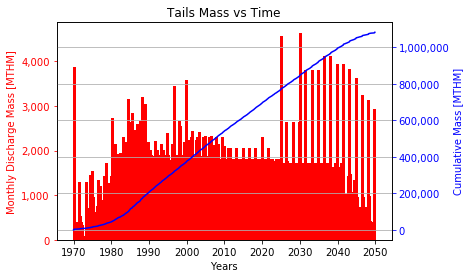
\includegraphics[scale=0.7]{./images/eu_future/tails.png}
	\end{center}
	\caption{This plot shows the timeseries of tails mass accumulation and discharge in the \gls{EU} nations.
			 Tails mass accumulation is fairly steady, with peaks occurring when
			 new reactors are deployed.}
	\label{fig:eu_tail}
\end{figure}

\begin{figure}[htbp!]
	\begin{center}
		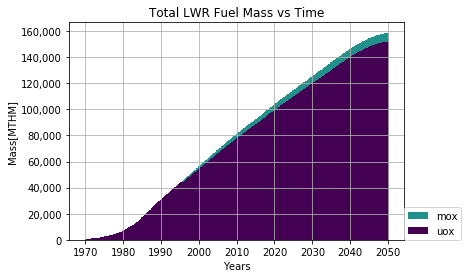
\includegraphics[scale=0.7]{./images/eu_future/total_fuel.png}
	\end{center}
	\caption{This plot shows the timeseries of total fuel usage in the \gls{EU} nations.}
	\label{fig:eu_fuel}
\end{figure}


\begin{figure}[htbp!]
	\begin{center}
			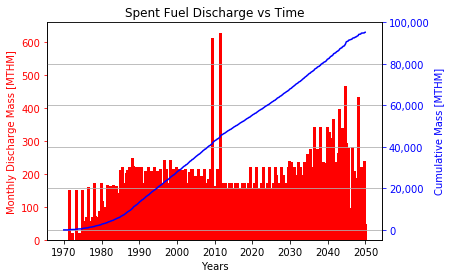
\includegraphics[scale=0.7]{./images/eu_future/snf_discharge.png}
	\end{center}
	\caption{This plot displays the timeseries of \gls{UNF} accumulation and discharge in the \gls{EU} nations.
			 The peaks are caused by decommissioning of reactors, where all the core is sent to the repository.}
	\label{fig:eu_snf}
\end{figure}
\FloatBarrier


\begin{table}[h]
	\centering
	\begin{tabular}{ccc}
		\hline
		\textbf{Isotope} & \textbf{Mass Fraction in Used Fuel [\%]} & \textbf{Quantity [t]} \\ \hline
		Total & 0.9358 & 1,325 \\ \hline
		Pu238 & 0.0111 & 15.72 \\ 
		Pu239 & 0.518 & 733.79 \\ 
		Pu240 & 0.232 & 328.64 \\ 
		Pu241 & 0.126 & 178.49 \\ 
		Pu242 & 0.0487 & 68.98 \\ \hline
	\end{tabular}
	\caption{Plutonium From Used Fuel}
	\label{tab:pu}
\end{table}


\Cref{tab:pu} lists the isotope, mass fraction,
and quantity of plutonium that can be obtained from the 2050 \gls{UNF} inventory.


\subsection{French \gls{SFR} Transition Scenario}

Reprocessing \gls{UNF} collected from all EU nations can start approximately
270 \glspl{SFR}, which is more than enough for two generations of 66GWe \gls{SFR}
fleet. With the \gls{SFR} breeding ratio of over one, France can transition into
a fully \gls{SFR} fleet without extra construction of \glspl{LWR}. 

From Varaine et al. \cite{varaine_pre-conceptual_2012}, a French
ASTRID-type \gls{SFR} of capacity 600 MWe needs $1.225$ tons of
plutonium a year, with an initial plutonium loading of $4.9$ tons. 
Thus, the number of \glspl{SFR} that can be loaded with the reprocessed
plutonium from \gls{UNF} can be estimated to $\frac{Pu \ from \ legacy \ \gls{UNF}}{4.9} \approx 270$ \glspl{SFR},
assuming infinite reprocessing and fabrication capacity as well as
abundant depleted uranium supply. 

Also, assuming that \gls{MOX} can be recycled indefinitely,
used \gls{MOX} from an ASTRID reactor contains enough plutonium to produce a \gls{MOX} fuel with
the same mass, if mixed with depleted uranium. For example,
used \gls{MOX} from an ASTRID reactor is assumed to be 12.6\% plutonium
in this simulation (see \cref{tab:comp}), whereas a fresh \gls{MOX} is 11\% plutonium.
Separating plutonium from used \gls{MOX} from
an ASTRID reactor can create \gls{MOX} of the mass of used \gls{MOX}.
The plutonium breeding ratio in this simulation is thus assumed to be
$\approx 1.145$.

\Cref{fig:fuel} shows \gls{MOX} loaded in the \glspl{SFR} per month.
The spikes are due to initial fuel demand for new deployment of \glspl{SFR}.
The initial loading of new \glspl{SFR} are done with the \gls{MOX} created
from legacy \gls{UNF}. Once there are enough amounts of extra plutonium creation
by deployed \glspl{SFR}, the legacy \gls{UNF} is no longer used. 

\begin{figure}[htbp!]
	\begin{center}
		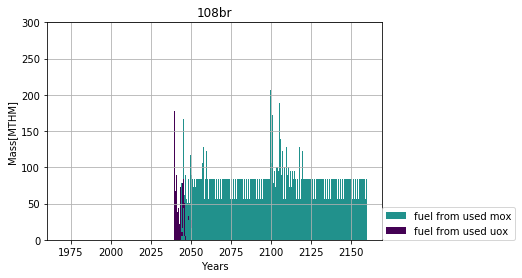
\includegraphics[scale=0.7]{./images/french-transition/where_fuel.png}
	\end{center}
	\caption{This plot displays the timeseries of fuel loaded into \glspl{SFR}.
			 The initial purple bars denote that the fuel is from reprocessing
			 the previously used \gls{UOX} inventory. The peaks coincide
			 with the new deployment of \glspl{SFR}.}
	\label{fig:fuel}
\end{figure}

\Cref{fig:reprocess_waste} shows the amount of reprocessing waste
(minor actinides, fission products) over time. The spikes in the 
waste discharge is due to large influx of used fuel from
decommissioned \glspl{SFR}.\Cref{fig:pu_no_cum} shows the separated plutonium discharge
per month from the reprocessing plant. The plutonium outflux
does not precisely follow the fuel demand because \Cyclus agents have
material buffers that store commodity fuel for later usage. 
\Cref{tab:sfr_sim_result} lists metrics obtained from the second simulation.

\begin{figure}[htbp!]
	\begin{center}
		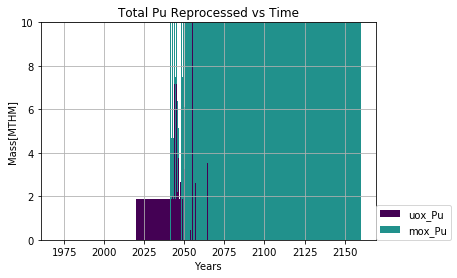
\includegraphics[scale=0.7]{./images/french-transition/pu.png}
	\end{center}
	\caption{This plot shows the separated plutonium discharge from the reprocessing plant.
			 The plutonium from reprocessing legacy fuel is a flat rectangle because the 
			 reprocessing throughput was set to 20 $\frac{tons}{month}$ to avoid reprocessing
			 all the legacy in one timestep.}
	\label{fig:pu_no_cum}
\end{figure}


\begin{figure}[htbp!]
	\begin{center}
		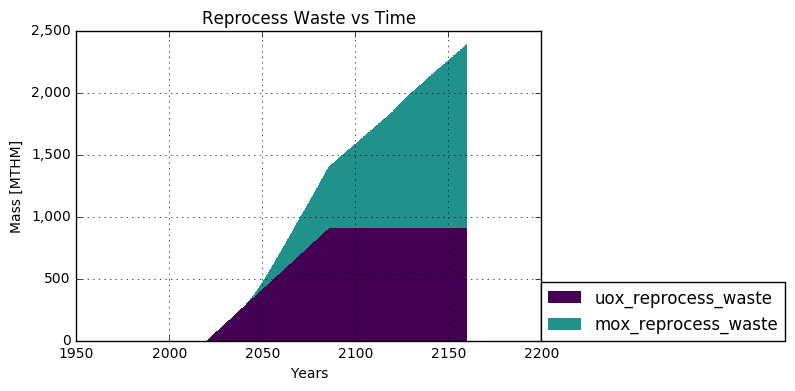
\includegraphics[scale=0.7]{./images/french-transition/reprocess_waste.png}
	\end{center}
	\caption{This plot displays raffinate discharge from each reprocessing plant.
			The plutonium from reprocessing legacy fuel is a flat rectangle because the 
			reprocessing throughput was set to 20 $\frac{tons}{month}$ to avoid reprocessing
			all the legacy in one timestep.}
	\label{fig:reprocess_waste}
\end{figure}


\begin{table}[h]
	\centering
	\scalebox{0.86}{
		\begin{tabular}{ccc}
			\hline
			\textbf{Category} & \textbf{Unit} & \textbf{Value}  \\ \hline
			Total MOX used & MTHM & 127,200  \\ 
			Total \glspl{SFR} Deployed & & 220 \\
			Total Plutonium Reprocessed & MTHM & 16,200 \\ 
			Total MOX from UOX Waste & MTHM & 6,570  \\ 
			Total MOX from MOX Waste & MTHM  & 121,070 \\ 
			Total Tails used & MTHM & 116,153 \\ 
			Total legacy UNF reprocessed & MTHM & 77,082 \\ 
			Total Reprocessed Uranium Stockpile & MTHM & 226,197 \\ 
			Total Reprocess Waste & MTHM & 16,352 \\ \hline
		\end{tabular}}
		\caption {Listed are the important metrics from the French transition to \gls{SFR} scenario.
				  The total legacy \gls{UNF} reprocessed is the amount of \gls{UNF} France would need
				  for a transition into a fully \gls{SFR} fleet. The tails used is almost a tenth
				  of the original tails inventory from the previous simulation.}
		\label{tab:sfr_sim_result}
\end {table}


